\documentclass[12pt]{article}

% Packages
\usepackage{lipsum}
\usepackage{setspace}
\usepackage{indentfirst}
\usepackage{geometry}
\usepackage[nonumberlist, toc]{glossaries}
\usepackage{graphicx}
\usepackage{caption}
\usepackage{subcaption}
\usepackage{tabularx}
\usepackage{booktabs}
\usepackage{enumitem}
\usepackage{xcolor}
\usepackage [autostyle, english = american]{csquotes}
\usepackage{fancyhdr}
\usepackage{amsmath}
\usepackage{cite}

% Formatting
\geometry{letterpaper, portrait, margin=.85in}
\MakeOuterQuote{"}
\pagestyle{fancy}
\lhead{MSXII Aerobody Flow Visualization} 
\rhead{Midnight Sun Solar Car Team}

\begin{document}

% Title Ppage
\begin{titlepage}
	\vspace*{2cm}
	\centering
	
\includegraphics[width=.25\textwidth]{./images/midnightSunLogoCircle.png}\par
	\vspace{1.5cm}
	{\scshape\LARGE Midnight Sun Solar Car Team \par}
	{\scshape\large University of Waterloo\par}
	\vspace{2.2cm}
	{\huge\bfseries MSXII Aerobody Flow Visualization\par}
	\vspace{0.2cm}
	\large Prepared for ME351 Project 1 
	\vspace{2.2cm}	
	\par Prepared by:\par
	Danyon Chu - 20563165\par
	Devon Copeland - 20553468\par
    
	\vspace{0.6cm} 
	\today\par
	\vfill
	www.uwmidsun.com \par
	(519) 888-4567 x 32978
\end{titlepage}

% Main Matter
\section{Background Information and Description of Flow}
Midnight Sun Twelve (MSXII) is a cruiser class, solar electric vehicle being designed with the goal of competing in the 2018 American Solar Challenge (ASC 2018) and the 2019 World Solar Challenge (WSC 2019). By definition, cruiser class solar vehicles must be multi-occupant and are designed with the intent of being more practical than a typical, challenger class solar car. The figure of merit for scoring for this class is predominantly efficiency based however teams are also awarded points for practicality and incorporating features that bring the car closer to what one might find in a consumer vehicle. Because of the unique challenges of this competition the areobody of MSXII must be designed to minimize drag while still keeping vehicle aesthetics and driver comfort in mind. This report summarizes an experiment that provides qualitative learnings regarding the flow of air over MSXII's aerobody by using a 3D printed scale model of the aerobody and a wind tunnel.

\section{Experimental Setup}
In order to visualize the flow of air over MSXII while driving, a wind tunnel was built and a 1:30 scale model of MSXII's aerobody was 3D printed. The wind tunnel was made using three boards of masonite and one piece of cast acrylic which provided a window such that the air flow could be seen from the outside. Opposite the acrylic, a dark coloured piece of paper was glued to the masonite on the inside of the tunnel to provide contrast against smoke. A fan with adjustable speed was then placed at one end of the tunnel to generate the airflow. Since the air flow downstream from the fan would likely be turbulent, the air was directed through a large bundle of straws before making contact with the car. The straws helped to create laminar airflow and removed disturbances from the fan. In order to visualize the airflow, a draft detector (smoke stick) was purchased to generate smoke. The smoke was then sucked from a reservoir outside the tunnel through a straw and then released just in front of the 3D printed model.

\begin{figure}[h!]
	\centering
	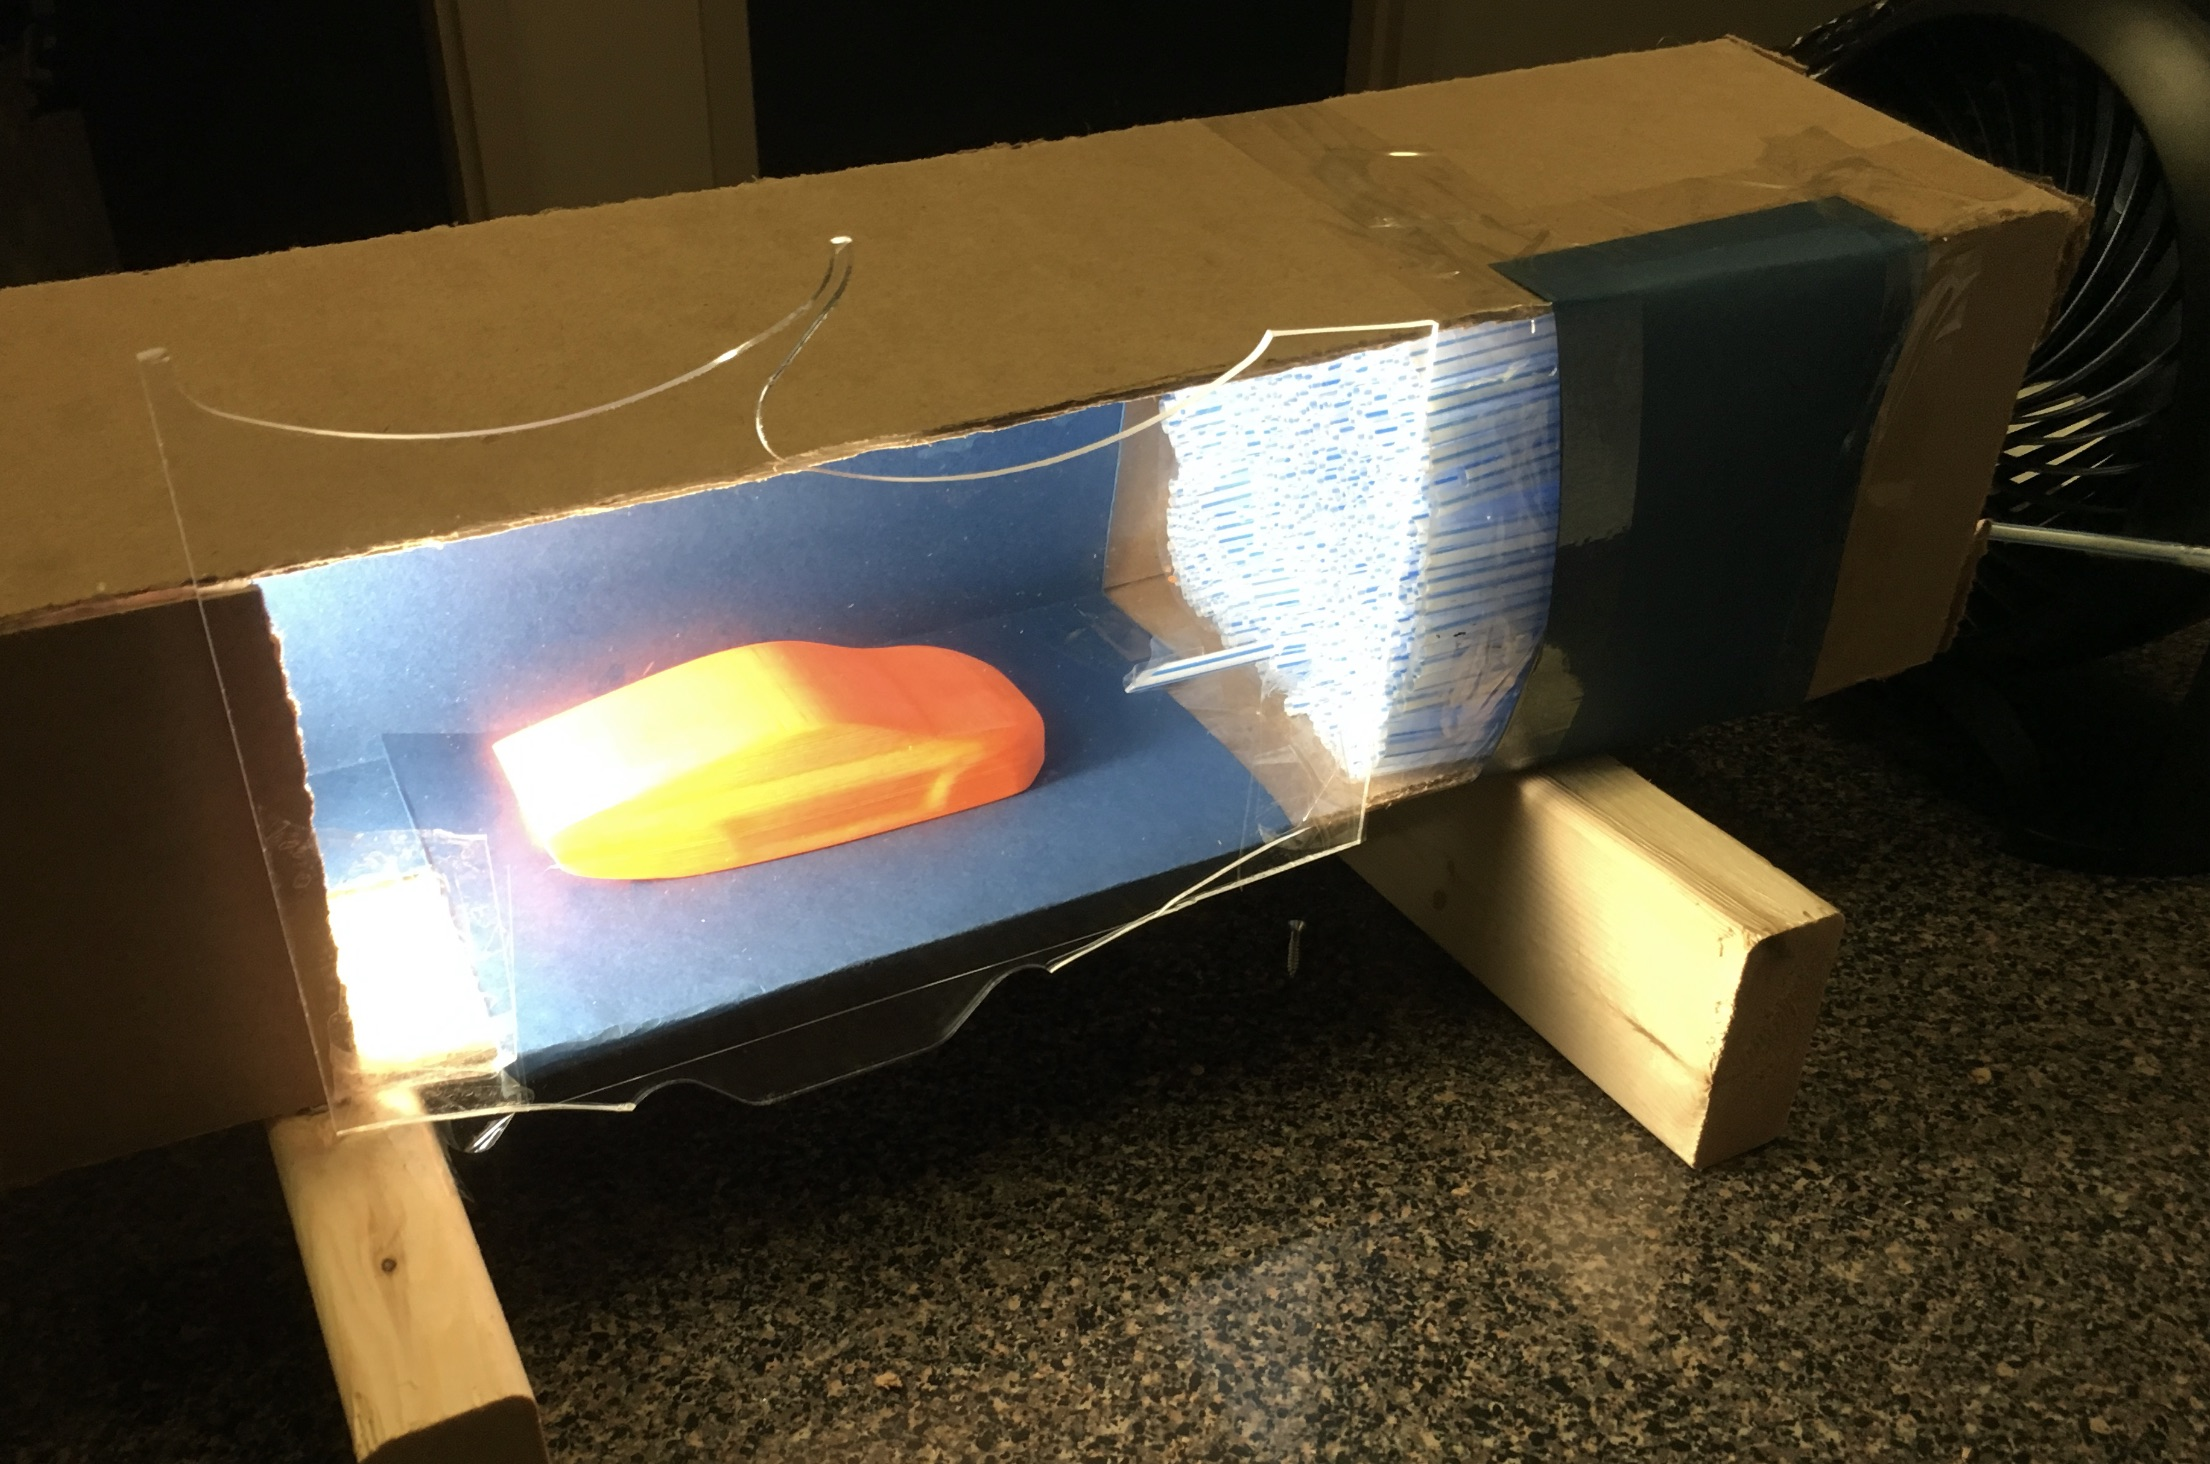
\includegraphics[width=.7\textwidth]{./images/setup1.jpg}
	\caption{Wind tunnel construction}
	\label{fig:setup1}
\end{figure}

\begin{figure}[h!]
	\centering
	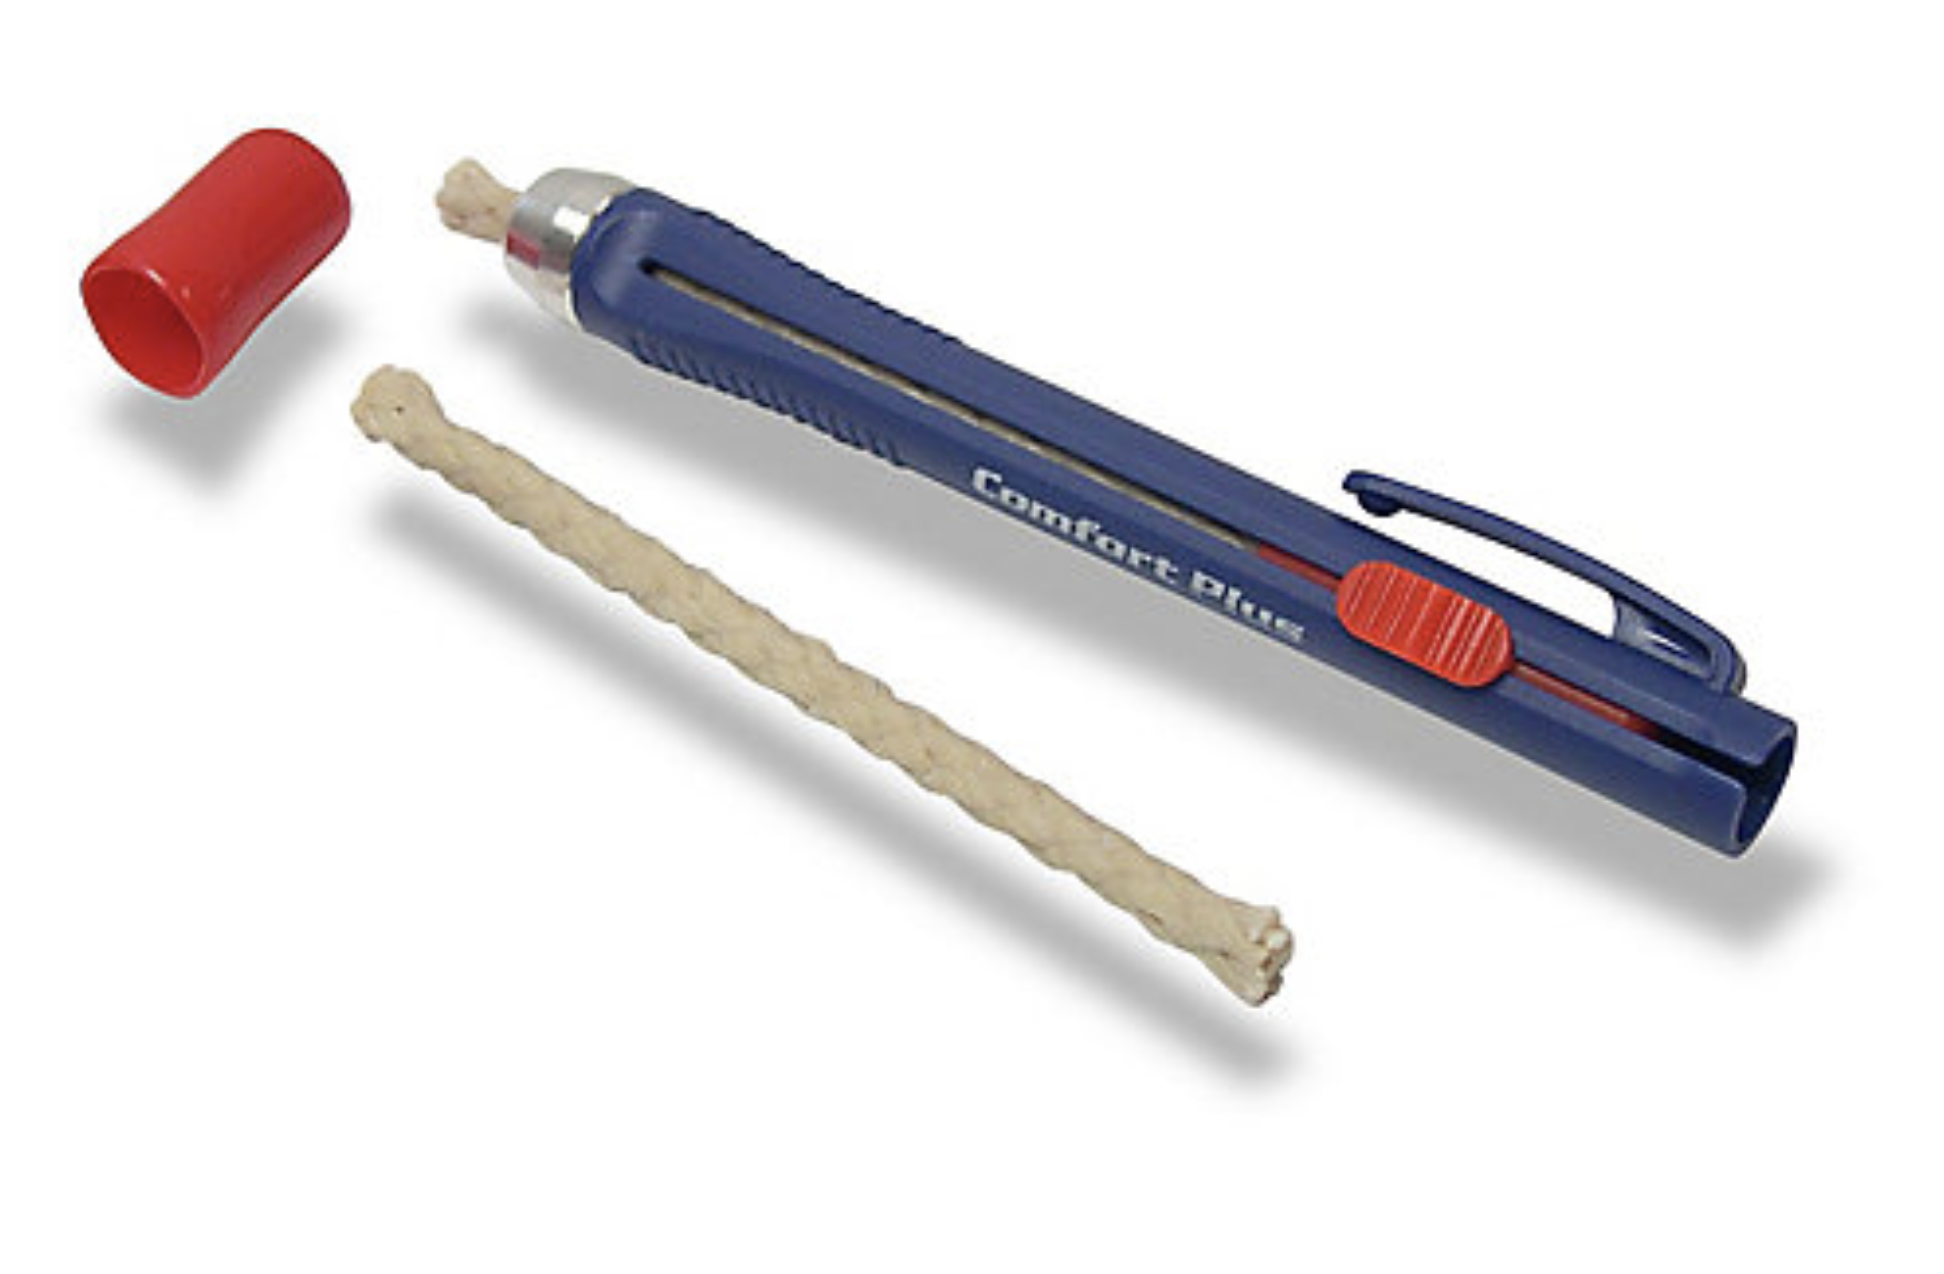
\includegraphics[width=.6\textwidth]{./images/draftDetector.png}
	\caption{The draft detector used to generate smoke}
	\label{fig:draftDetector}
\end{figure}

\begin{figure}[h!]
	\centering
	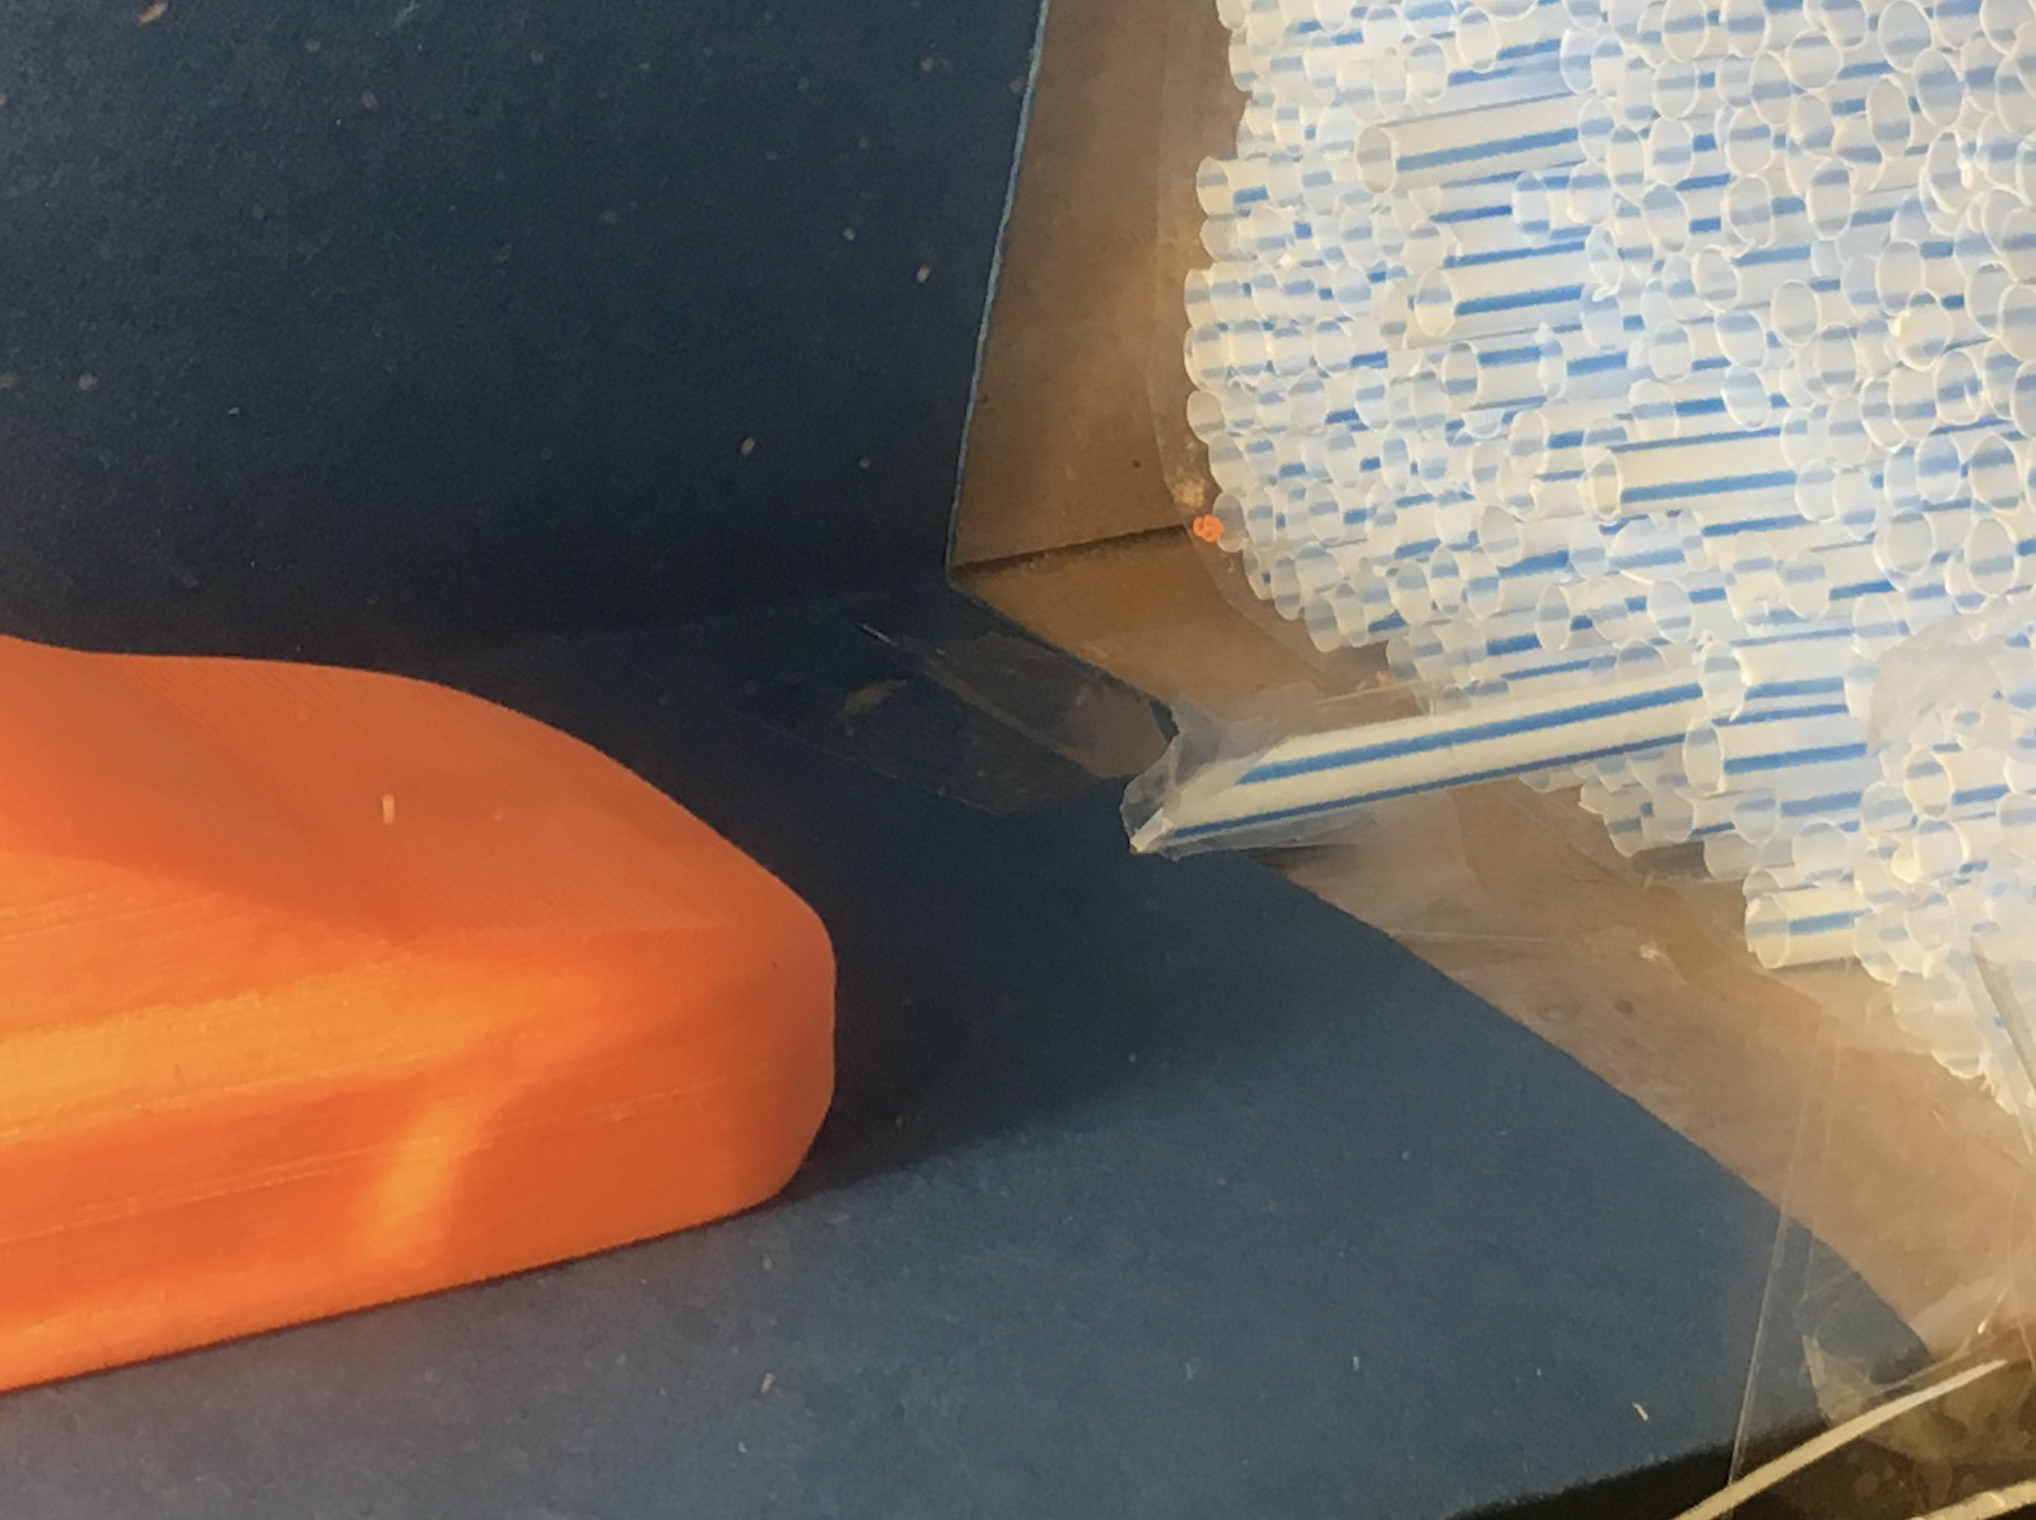
\includegraphics[width=.7\textwidth]{./images/setup2.jpg}
    \captionsetup{justification=centering,margin=2cm}
	\caption{Smoke is transported through a straw from a reservoir outside the tunnel and released directly in front of the 3D printed part}
	\label{fig:setup2}
\end{figure}

\begin{figure}[h!]
	\centering
	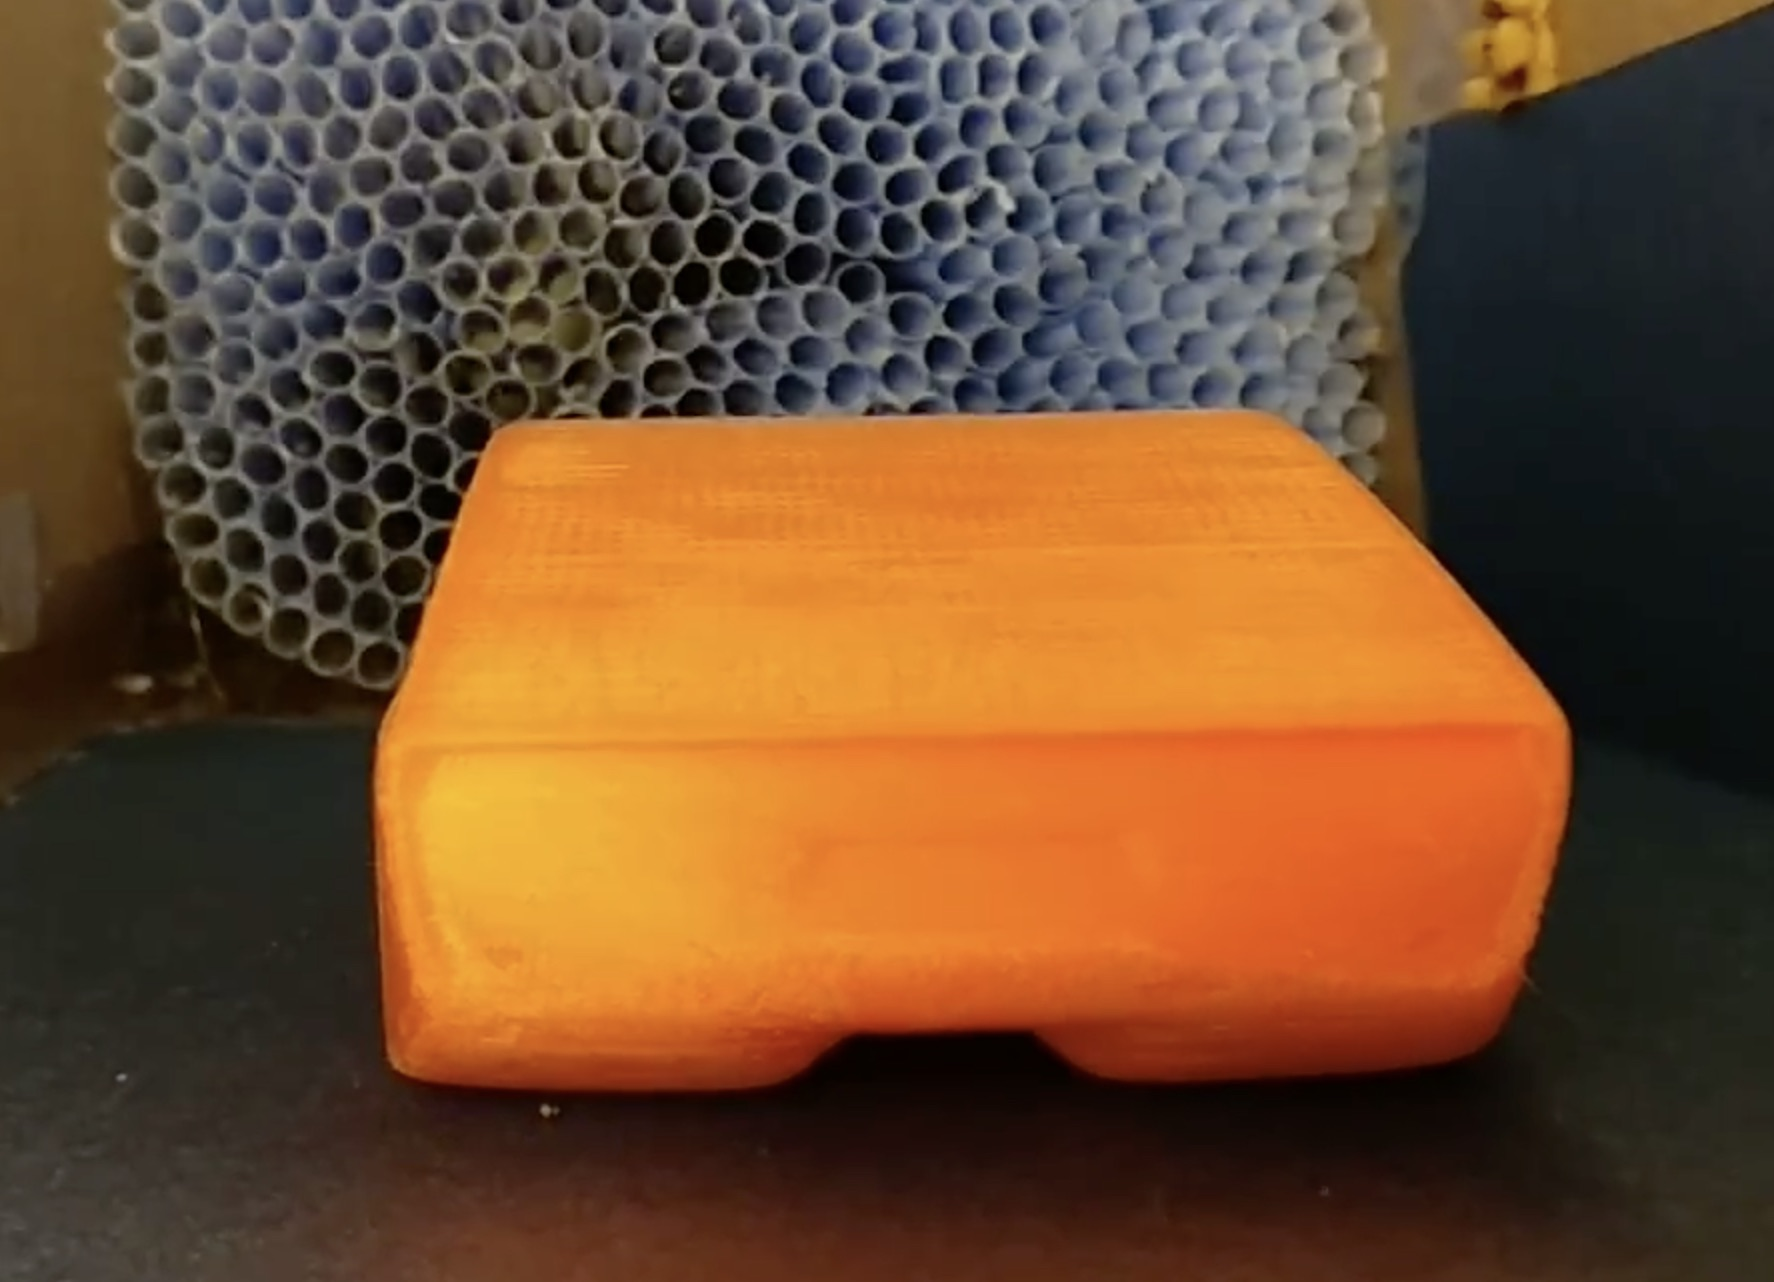
\includegraphics[width=.7\textwidth]{./images/setup3.jpg}
    \captionsetup{justification=centering,margin=2cm}
	\caption{Straws placed downstream of the fan help to remove turbulence from the moving air column}
	\label{fig:setup3}
\end{figure}

\section{Observations}
Several observations can be made based on the flow of smoke over the 3D printed aerobody. One such observation relates to the experimental setup. As noted in the previous section, several steps were taken to ensure that the air flow in the wind tunnel was laminar; including the wall of straws and adjustable speed on the fan. While conducting the experiment, the speed of the fan was reduced to it's lowest setting and the smoke in the wind tunnel created a fairly clean streakline before striking the body of the vehicle. This indicates that these design considerations have helped accomplished the goal of reducing turbulence in the airflow. These observations also coincide with trends in the literature; where higher velocity air flows tend to be more turbulent than lower velocity air flows and small diameter flows (like that of the straws) tend to be more laminar. Explained differently, based on the the governing equation for Reynolds Number, speed plays a direct roll in determining whether a flow is turbulent or laminar:

\begin{center}
$Re = \frac{VL}{\mu}$ 
\end{center}

where: V = velocity, L = length, $\mu$ = kinematic velocity and that a high Re is an indicator of turbulent air flow.

Another notable observation relates to the position from which the smoke was released. Through experimentation it was determined that releasing the smoke from a small aperture led to a cleaner streakline. For this reason, the smoke from the draft detector was fed into the wind tunnel through a single straw connected to a reservoir rather than simply through the fan. 

A third key observation relates to the flat area on the rear of the car that was originally designed to accommodate a road legal license plate. This flat area was predicted to lead to a less aerodynamic design. Although an eddy can still be seen at the rear of the vehicle in Figure \ref{fig:sideFlow}, the flow moving underneath the car through the catamaran seen in Figure \ref{fig:rearFlow} seemed to help mitigate or reduce the amount of negative pressure and eddies seen behind the vehicle.

Overall, the most important observation that the custom wind tunnel has enabled is a high level view of the flow separation across the vehicle. Where possible, MSXII was designed to emulate the optimal teardrop shape while still resembling an actual vehicle. In doing so a number of simulations were done to try to optimize certain features for efficiency. By providing a physical representation of the streaklines over the car, this study has helped to corroborate data from CFD and draw connections between these simulations and the real world.\\

To view a video of the experiment, please visit: www.tinyurl.com/msxiiflow

\begin{figure}[h!]
	\centering
	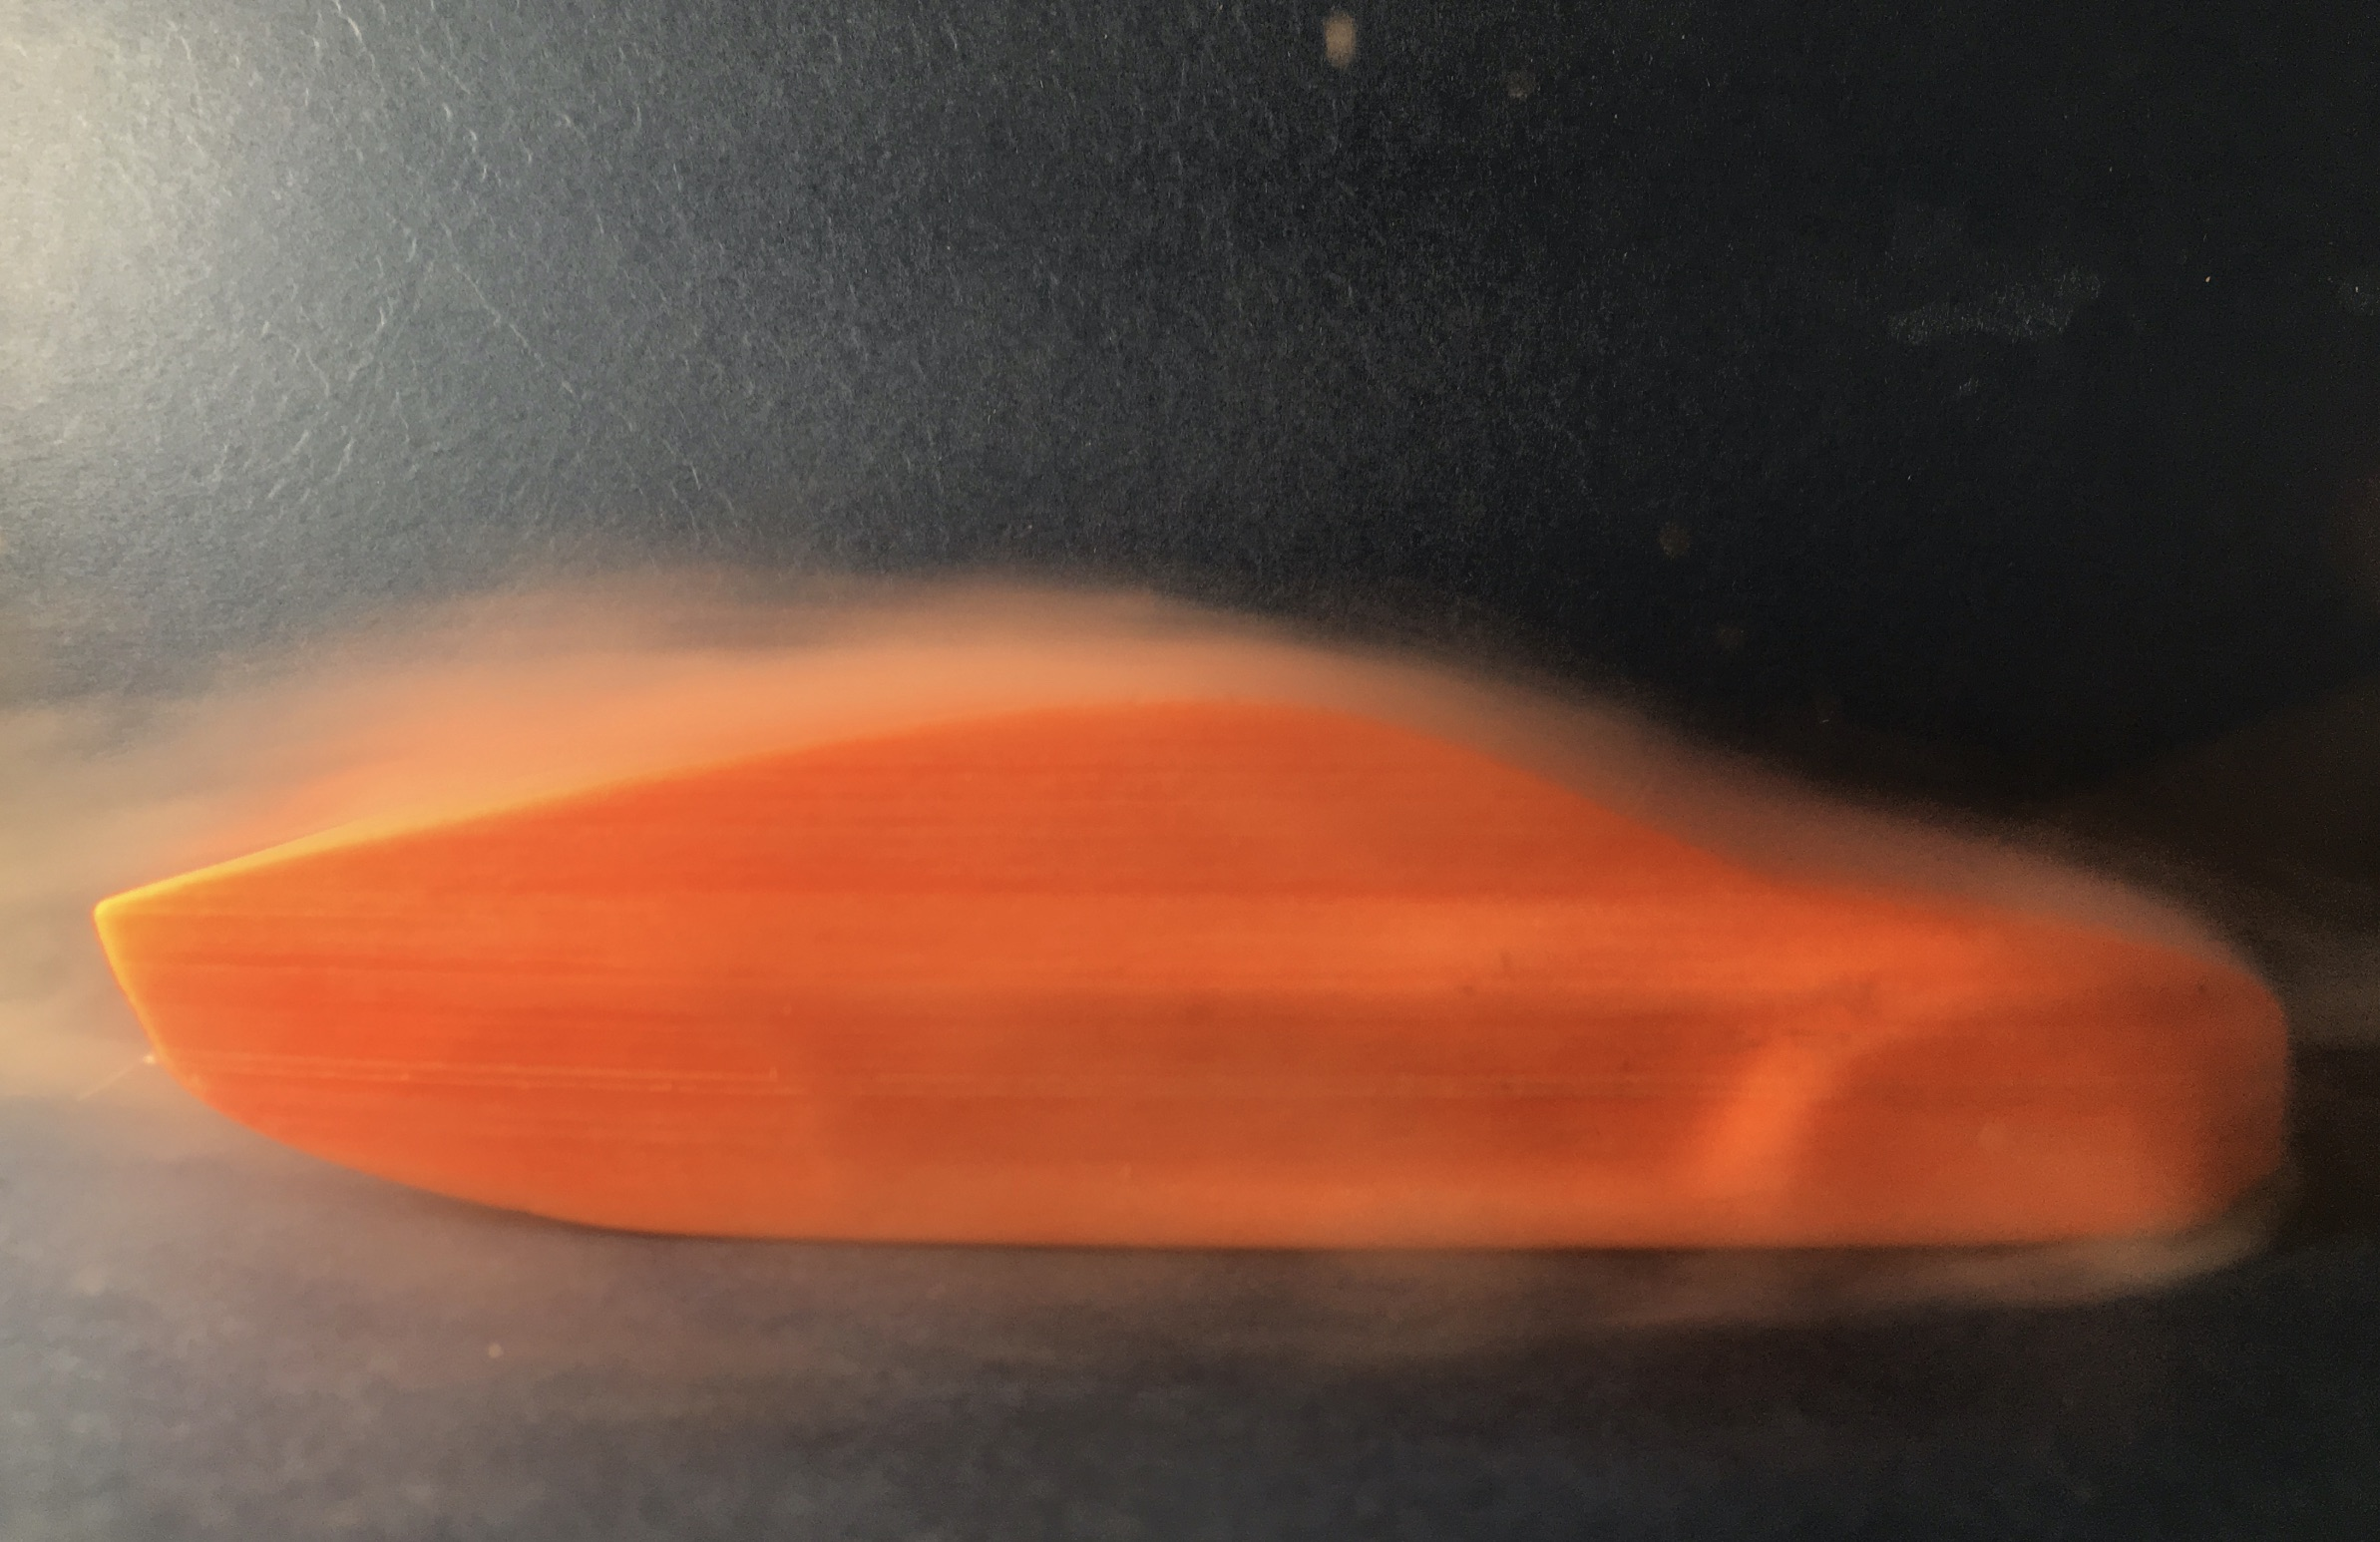
\includegraphics[width=.7\textwidth]{./images/sideFlow1.jpg}
    \captionsetup{justification=centering,margin=2cm}
	\caption{Laminar air stream over the MSXII model as seen from the side view}
	\label{fig:sideFlow}
\end{figure}

\begin{figure}[h!]
	\centering
	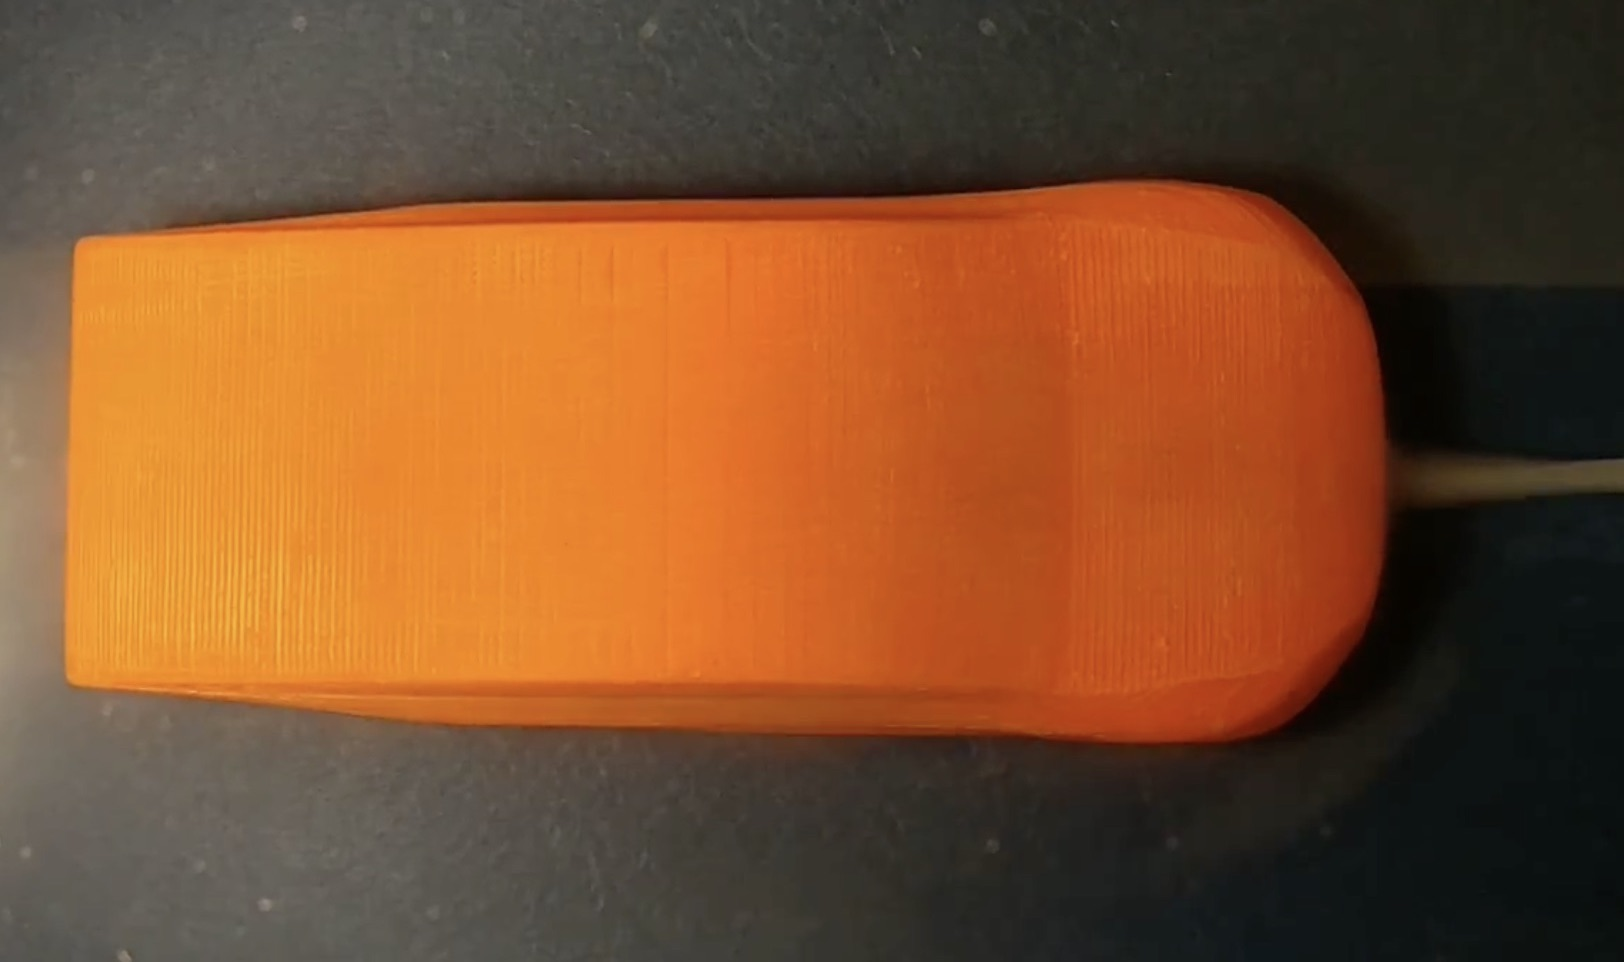
\includegraphics[width=.7\textwidth]{./images/topFlow1.jpg}
    \captionsetup{justification=centering,margin=2cm}
	\caption{Laminar air stream over the MSXII model as seen from the top view}
	\label{fig:topFlow}
\end{figure}

\begin{figure}[h!]
	\centering
	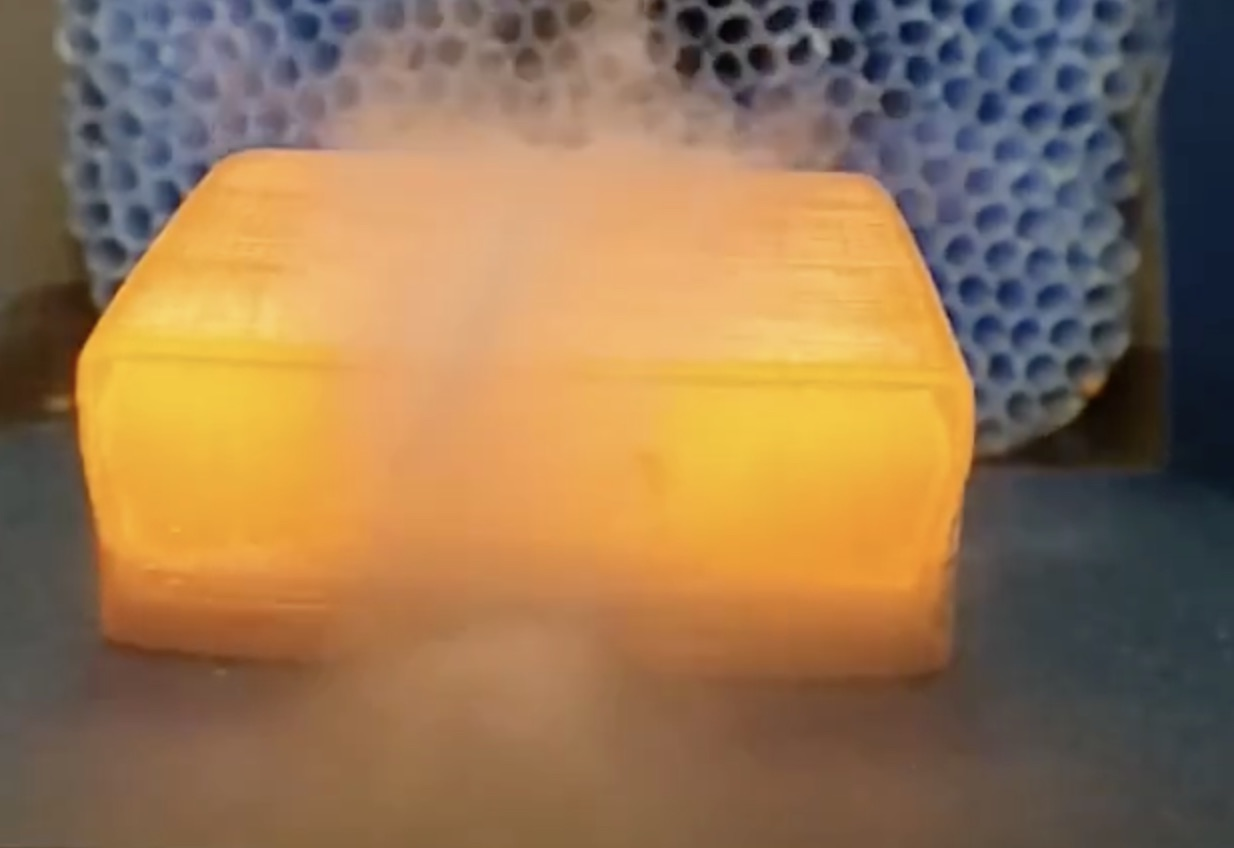
\includegraphics[width=.7\textwidth]{./images/rearFlow1.jpg}
    \captionsetup{justification=centering,margin=2cm}
	\caption{Laminar air stream over the MSXII model as seen from the rear view}
	\label{fig:rearFlow}
\end{figure}


% Bibliography
\pagebreak
\bibliography{./latex/bib}{}
\bibliographystyle{plain}

\end{document}
